% Options for packages loaded elsewhere
\PassOptionsToPackage{unicode}{hyperref}
\PassOptionsToPackage{hyphens}{url}
%
\documentclass[
]{book}
\usepackage{lmodern}
\usepackage{amssymb,amsmath}
\usepackage{ifxetex,ifluatex}
\ifnum 0\ifxetex 1\fi\ifluatex 1\fi=0 % if pdftex
  \usepackage[T1]{fontenc}
  \usepackage[utf8]{inputenc}
  \usepackage{textcomp} % provide euro and other symbols
\else % if luatex or xetex
  \usepackage{unicode-math}
  \defaultfontfeatures{Scale=MatchLowercase}
  \defaultfontfeatures[\rmfamily]{Ligatures=TeX,Scale=1}
\fi
% Use upquote if available, for straight quotes in verbatim environments
\IfFileExists{upquote.sty}{\usepackage{upquote}}{}
\IfFileExists{microtype.sty}{% use microtype if available
  \usepackage[]{microtype}
  \UseMicrotypeSet[protrusion]{basicmath} % disable protrusion for tt fonts
}{}
\makeatletter
\@ifundefined{KOMAClassName}{% if non-KOMA class
  \IfFileExists{parskip.sty}{%
    \usepackage{parskip}
  }{% else
    \setlength{\parindent}{0pt}
    \setlength{\parskip}{6pt plus 2pt minus 1pt}}
}{% if KOMA class
  \KOMAoptions{parskip=half}}
\makeatother
\usepackage{xcolor}
\IfFileExists{xurl.sty}{\usepackage{xurl}}{} % add URL line breaks if available
\IfFileExists{bookmark.sty}{\usepackage{bookmark}}{\usepackage{hyperref}}
\hypersetup{
  pdftitle={Matematika Bisnis},
  pdfauthor={Bakti Siregar, S.Si., M.Sc},
  hidelinks,
  pdfcreator={LaTeX via pandoc}}
\urlstyle{same} % disable monospaced font for URLs
\usepackage{longtable,booktabs}
% Correct order of tables after \paragraph or \subparagraph
\usepackage{etoolbox}
\makeatletter
\patchcmd\longtable{\par}{\if@noskipsec\mbox{}\fi\par}{}{}
\makeatother
% Allow footnotes in longtable head/foot
\IfFileExists{footnotehyper.sty}{\usepackage{footnotehyper}}{\usepackage{footnote}}
\makesavenoteenv{longtable}
\usepackage{graphicx,grffile}
\makeatletter
\def\maxwidth{\ifdim\Gin@nat@width>\linewidth\linewidth\else\Gin@nat@width\fi}
\def\maxheight{\ifdim\Gin@nat@height>\textheight\textheight\else\Gin@nat@height\fi}
\makeatother
% Scale images if necessary, so that they will not overflow the page
% margins by default, and it is still possible to overwrite the defaults
% using explicit options in \includegraphics[width, height, ...]{}
\setkeys{Gin}{width=\maxwidth,height=\maxheight,keepaspectratio}
% Set default figure placement to htbp
\makeatletter
\def\fps@figure{htbp}
\makeatother
\setlength{\emergencystretch}{3em} % prevent overfull lines
\providecommand{\tightlist}{%
  \setlength{\itemsep}{0pt}\setlength{\parskip}{0pt}}
\setcounter{secnumdepth}{5}
\usepackage{booktabs}
\usepackage{amsthm}
\makeatletter
\def\thm@space@setup{%
  \thm@preskip=8pt plus 2pt minus 4pt
  \thm@postskip=\thm@preskip
}
\makeatother
\usepackage[]{natbib}
\bibliographystyle{apalike}

\title{Matematika Bisnis}
\author{Bakti Siregar, S.Si., M.Sc}
\date{September 09, 2020}

\begin{document}
\maketitle

{
\setcounter{tocdepth}{1}
\tableofcontents
}
\hypertarget{selamat-datang}{%
\chapter*{Selamat Datang!}\label{selamat-datang}}
\addcontentsline{toc}{chapter}{Selamat Datang!}

\begin{center}\rule{0.5\linewidth}{0.5pt}\end{center}

\begin{center}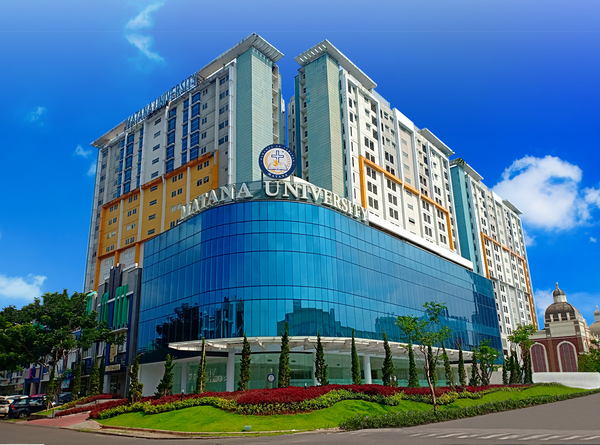
\includegraphics[width=0.5\linewidth]{images/cover} \end{center}

Program Studi Statistika
Fakultas Science, Technology, Engineering, and Mathematics (STEM)
Tangerang, Banten
Info: siregarbakti@gmail.com

\hypertarget{kata-pengantar}{%
\section*{Kata Pengantar}\label{kata-pengantar}}
\addcontentsline{toc}{section}{Kata Pengantar}

Buku ini dituliskan untuk mempermudah proses pembelajaran Matematika Bisnis di Universitas Matana. Materi dikemas secara khusus dalam bentuk e-book yang mudah dipahami dan dapat dibaca melalui PC maupun Tablet anda dimanapun-kapanpun dengan akses internet.

Adapun Materi yang akan dibahas dalam buku ini adalah sebagai berikut:

\begin{itemize}
\tightlist
\item
  Minggu 1 \textasciitilde{} Pengenalan Matematika Bisnis
\item
  Minggu 2 \textasciitilde{} Dasar-dasar Matematika Bisnis
\item
  Minggu 3 \textasciitilde{} Aplikasi Manajemen Bisnis Umum
\item
  Minggu 4 \textasciitilde{} Sumber Daya Manusia dan Aplikasi Ekonomi
\item
  Minggu 5 \textasciitilde{} Dasar-dasar Pemasaran dan Akuntansi
\item
  Minggu 6 \textasciitilde{} Aplikasi Pemasaran
\item
  Minggu 7 \textasciitilde{} Aplikasi Akuntansi
\item
  Minggu 8 \textasciitilde{} Ujian Tengah Semester
\item
  Minggu 9 \textasciitilde{} Bunga Sederhana- Bekerja Dengan Pembayaran Tunggal dan Aplikasi
\item
  Minggu 10 \textasciitilde{} Bunga Majemuk- Bekerja Dengan Pembayaran Tunggal
\item
  Minggu 11 \textasciitilde{} Bunga Majemuk- Aplikasi yang Melibatkan Pembayaran Tunggal
\item
  Minggu 12 \textasciitilde{} Bunga Majemuk- Anuitas
\item
  Minggu 13 \textasciitilde{} Bunga Majemuk- Aplikasi Khusus Anuitas
\item
  Minggu 14 \textasciitilde{} Memahami Amortisasi dan Aplikasinya
\item
  Minggu 15 \textasciitilde{} Obligasi dan Dana Tenggelam
\item
  Minggu 16 \textasciitilde{} Ujian Akhir
\end{itemize}

\hypertarget{tentang-penulis}{%
\section*{Tentang Penulis}\label{tentang-penulis}}
\addcontentsline{toc}{section}{Tentang Penulis}

Bakti Siregar adalah lulusan Universitas Sumatera Utara (USU), Jurusan Matematika. Setelah meluluskan S1 nya di tahun 2013, langsung mendapatkan perkerjaan di PT. Asuransi Sinar Mas sebagai Underwriter Managament Trainee. Di tahun 2014 beranjak ke perusahaan Multifinance sebagai Credit Analyst. Tak lama berselang, Beliau memutuskan untuk melanjutkan studinya dan berhasil memperoleh gelar Masternya dengan beasiswa yang diperoleh dari National Sun Yat-sen University (NSYSU-Taiwan), Jurusan Matematika Terapan Sains Data (Data Science).

Selain menjadi seseorang yang berfrofesi sebagai Data Scientist, beliau juga menjadi dosen Matematika dan Statistik, Prodi Statistika Universitas Matana, Tengerang. Di universitas ini Bakti siregar telah mengajar Matematika Bisnis dan Keuangan, serta Statistik Bisnis dan Metode Kuantitatif selama 2 tahun terakhir. Dia adalah instruktur berdedikasi yang tertarik untuk membantu siswanya berhasil melalui pengajaran multi-media yang melibatkan PowerPoint, video, diskusi dalam kelas, bacaan, perangkat lunak online, dan praktik pekerjaan rumah. Dia secara teratur memfasilitasi kursus kuantitatif ini dan memimpin tim instruktur. Anda mungkin pernah bertemu Bakti Siregar di berbagai simposium matematika dan statistik yang diadakan di seluruh Indonesia (dan dunia). Dia telah berkontribusi pada berbagai publikasi matematika untuk penerbit besar sehubungan dengan ulasan, pengembangan PowerPoint, penulisan algoritmik online, pemeriksaan teknis, dan penulisan bersama buku teks. Buku ini adalah salah satu usaha pertama Bakti Siregar dalam penulisan tunggal.

Bakti Siregar tinggal di Bekasi, Jawa barat, Indonesia, bersama adik laki-lakinya yang sedang menempuh perkuliahan di program studi Manajemen. Ketika dia tidak mengajar, dia suka berlibur di iklim Sejuk seperti Puncak, Bogor, dan Bandung bersama sanak saudaranya.

\begin{center}\rule{0.5\linewidth}{0.5pt}\end{center}

Bakti Siregar, S.Si., M.Sc
Email: \href{mailto:siregarbakti@gmail.com}{\nolinkurl{siregarbakti@gmail.com}} / \href{mailto:siregar.bakti@matanauniversity.ac.id}{\nolinkurl{siregar.bakti@matanauniversity.ac.id}}
Github: \url{https://github.com/Bakti-Siregar}
LinkedIn: \url{https://www.linkedin.com/in/bakti-siregar-15955480/}

\hypertarget{Pendahuluan}{%
\chapter{Pendahuluan}\label{Pendahuluan}}

\begin{center}\rule{0.5\linewidth}{0.5pt}\end{center}

Bab ini, sedang dalam proses penulisan. Akan segera update. Bagian ini hanya membahas mengenai kontrak kuliah, rencana pembelajaran, dan tinjauan penilaian yang dilakukan dosen pengampu.

\hypertarget{Dasar-Matematika-Bisnis}{%
\chapter{Dasar Matematika Bisnis}\label{Dasar-Matematika-Bisnis}}

\begin{center}\rule{0.5\linewidth}{0.5pt}\end{center}

Kemana anda bisa pergi dalam hidup dan tidak mengenal angka dan matematika? Bahkan saat anda sedang mencari tahu harga suatu produk (termasuk pengiriman) di Lazada, Tokopedia, Traveloka, dll, begitupun saat mengatur pemasukan dan pengeluaran di rekening bank anda, dalam hal ini diperlukan keterampilan matematika sederhana dari pendidikan dasar dan hingga pendidikan menengah. Berikut ini diulas beberapa contoh sederhana mengenai penerapan matematika yang anda lakukan setiap hari:

\begin{itemize}
\tightlist
\item
  Di toko bahan makanan, anda seringkali membandingkan produk untuk menghitung nilai terbaik. Satu merek keripik kentang dijual seharga \(\$ 3,99\) untuk 300 g, sedangkan merek yang sama memuaskannya di sampingnya seharga \(\$ 3,49\) untuk 250 g. Mana yang menawarkan nilai lebih baik?
\item
  Jika anda adalah penggemar olahraga, anda tahu banyak statistik tentang pemain dan tim favorit anda. Banyak yang datang dalam bentuk persentase, seperti lemparan tiga poin untuk bintang NBA atau menyimpan persentase untuk penjaga gawang NHL. Apa sebenarnya arti persentase tersebut?
\item
  Banyak majikan membayar bonus. Mungkin di perusahaan anda, manajer mendapatkan bonus dua kali lebih besar daripada karyawan. Perusahaan anda memiliki lima manajer dan 25 karyawan. Jika mengumumkan bonus total \(\$ 35.000,\) berapa bagian anda sebagai karyawan?
\end{itemize}

Sadar atau tidak Matematika dan angka mengelilingi anda di dunia bisnis, termasuk saat anda harus membaca banyak laporan numerik, menafsirkan bagaimana angka-angka itu cocok, dan membuat laporan anda sendiri yang menunjukkan metrik seperti proyeksi penjualan dan laba. Diluar pekerjaan, anda juga harus mengelola pendapatan dan membayar tagihan anda. Ini adalah masalah matematika yang mungkin anda pecahkan setiap hari, memastikan bahwa uang yang mengalir keluar dari rekening bank anda tidak melebihi uang yang mengalir masuk. Untuk membeli bahan makanan, liburan, atau hiburan, dalam hal ini ada perlu untuk mempertimbangkan prioritas utama.

Bab ini mengulas tentang keterampilan matematika dasar yang menjadi acuan penting di bab-bab selanjutnya. Beberapa contoh akan dijelaskan secara rinci, sementara yang lain akan diseerahkan kepada anda untuk menyelesaikan bab ini secara mandiri. Bagaimanapun, bab ini penting dan harus digunakan untuk menguji kemampuan dasar anda. Olehkarena itu, pelajarilah bab ini dengan percaya diri, dan jika anda menemui kesulitan, pastikan anda menguasai konsep sebelum melanjutkan ke bab berikutnya.

\hypertarget{urutan-perhitungan}{%
\section{Urutan Perhitungan}\label{urutan-perhitungan}}

Andaikan baru saja anda memenangkan \(\$ 50.000\) dalam sebuah undian, Yeah\ldots{} Selamat untuk Anda! Tetapi sebelum dapat mengklaimnya, anda diminta untuk menjawab pertanyaan pengujian keterampilan matematika, dan tidak ada kalkulator yang diizinkan. Setelah anda menyerahkan tiket kemenangan ke agen penukaran, dia memberikan pertanyaan pengujian keterampilan terbatas waktu: 2 × 5 + 30 ÷ 5. Saat waktu dihitung mundur, anda pasti mempertimbangkan berbagai kemungkinan. Apakah jawabannya 8, 14, 16, atau sama sekali berbeda? Bukankah sangat buruk kehilangan \$ 50.000 karena anda tidak dapat menjawab pertanyaan itu! Jika anda menemukan solusinya adalah 16, anda berada di jalan yang benar. Sebaliknya jika anda memperoleh jawaban berbeda, inilah saat yang tepat untuk meninjau ulang cara anda melakukan perhitungan.

Dalam buku ini akan diperkenalkan operasi perhitungan matematika dengan menggunakan EXcel yang mungkin saja memiliki kesamaan dengan beberapa Kalkulator atau Applikasi. Operator yang anda gunakan dalam Excel adalah factor yang paling krusial saat melakukan penghitungan yang ingin Anda lakukan pada elemen suatu rumus. Excel mengikuti aturan matematika umum untuk penghitungan, yaitu Tanda Kurung (Parentheses), Eksponen (Exponents), Perkalian dan Pembagian (Multiplication and Division), serta Penambahan dan Pengurangan (Addition and Subtraction). Perlu dicatat bahwa penggunaan tanda kurung memungkinkan anda mengubah urutan penghitungan tersebut.

\hypertarget{operator-aritmetika}{%
\section{Operator Aritmetika}\label{operator-aritmetika}}

Untuk melakukan operasi matematika dasar, seperti penambahan, pengurangan, perkalian, atau pembagian; menggabungkan angka; dan menghasilkan nilai numerik, anda dapat menggunakan operator aritmetika berikut ini dalam Excel.

\begin{figure}

{\centering 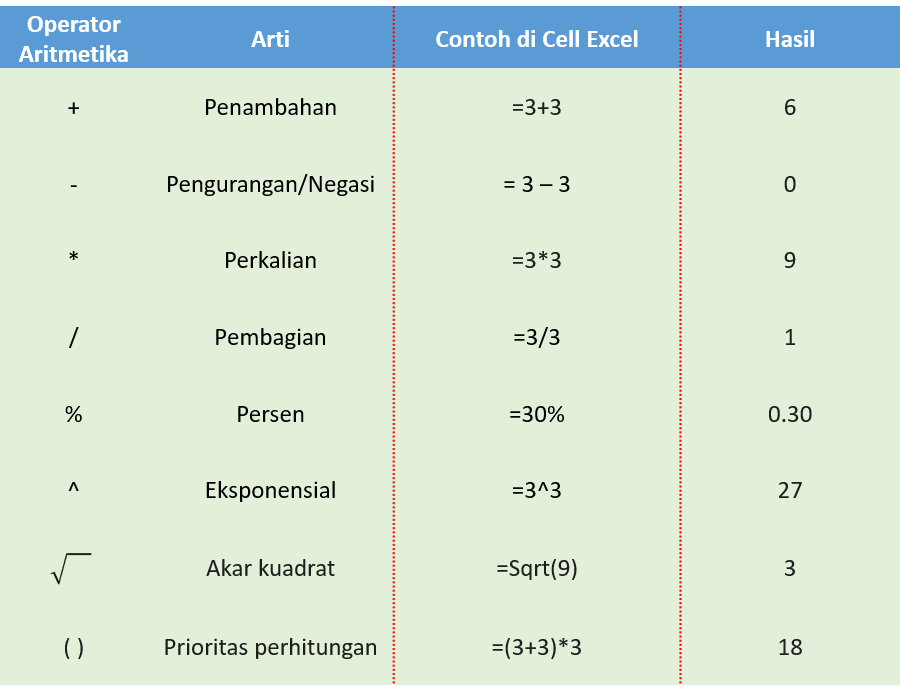
\includegraphics[width=0.75\linewidth]{images/aritmatika} 

}

\caption{Operator Aritmetika}\label{fig:aritmatika}
\end{figure}

\textbf{Catatan:} () atau {[}{]} atau \{\} Secara berurutan, ini dikenal sebagai tanda kurung bulat, persegi, dan keriting.

\hypertarget{operator-perbandingan}{%
\section{Operator Perbandingan}\label{operator-perbandingan}}

Saat dua nilai dibandingkan dengan menggunakan operator ini, hasilnya adalah nilai logika---TRUE atau FALSE. Anda juga dapat membandingkan dua nilai dengan operator berikut dalam Excel.

\begin{figure}

{\centering 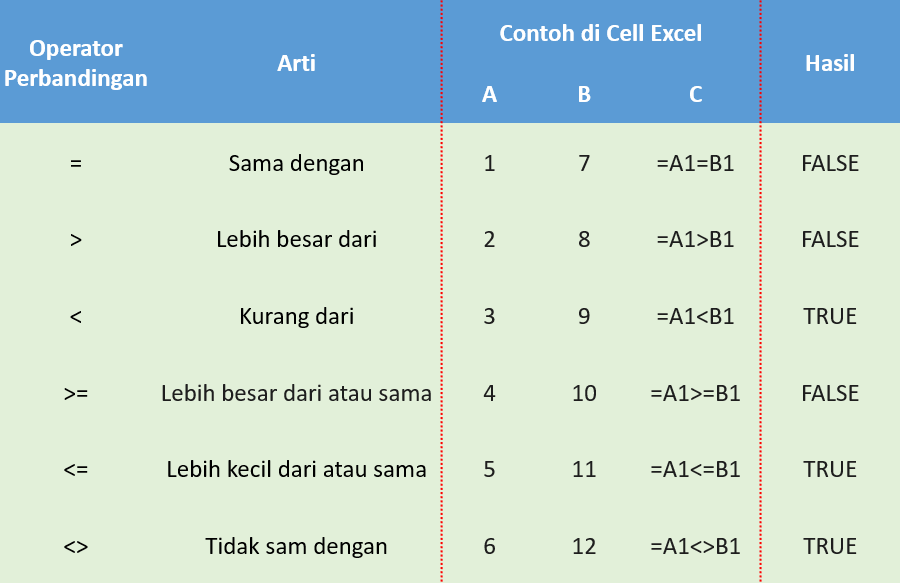
\includegraphics[width=0.75\linewidth]{images/perbandingan} 

}

\caption{Operator Perbandingan}\label{fig:perbandingan}
\end{figure}

\hypertarget{operator-referensi}{%
\section{Operator Referensi}\label{operator-referensi}}

Pada bagian ini ada diharapakan untuk dapat menggunakan penggabungan rentang sel untuk perhitungan dengan operator dalam Excel.

\begin{figure}

{\centering 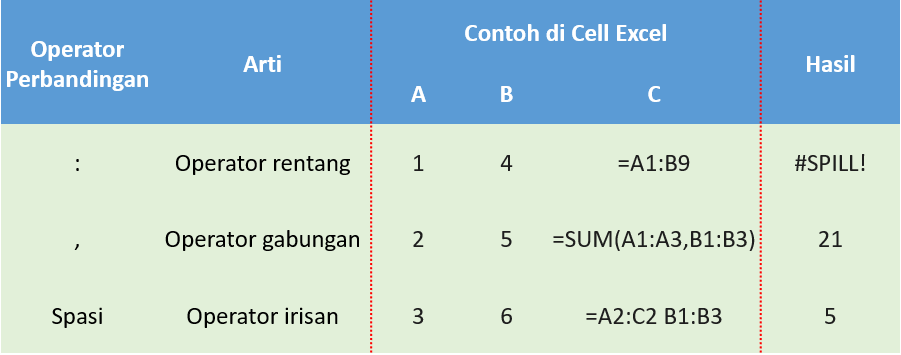
\includegraphics[width=0.75\linewidth]{images/referensi} 

}

\caption{Operator Referensi}\label{fig:referensi}
\end{figure}

\textbf{Catatan:} Kesalahan \#SPILL dikembalikan saat rumus mengembalikan beberapa hasil, dan Excel tidak bisa mengembalikan hasil ke Cell. Operator rentang \texttt{:} ini tidak dapat berdiri sendiri.

\hypertarget{sistem-persamaan-linear}{%
\section{Sistem Persamaan Linear}\label{sistem-persamaan-linear}}

Sistem persamaan linear adalah persamaan-persamaan linear yang dikorelasikan untuk membentuk suatu sistem. Sistem persamaannya bisa terdiri dari satu variabel, dua variabel atau lebih. Dalam bahasan ini, kita hanya membahas sistem persamaan linear dengan dua dan tiga variabel.

\hypertarget{sistem-persamaan-linear-dua-variabel-spldv}{%
\subsection{Sistem Persamaan Linear Dua Variabel (SPLDV)}\label{sistem-persamaan-linear-dua-variabel-spldv}}

Sistem persamaan linear dua variabel adalah sistem persamaan linear yang terdiri dari dua persamaan dimana masing-masing persamaan memiliki dua variabel. Bentuk umum SPLDV dengan variabel x dan y:

Sebagai contoh ada dua persamaan linier yaitu

\begin{itemize}
\tightlist
\item
  \(y_1 = 10 -2x\) dan
\item
  \(y_2 = 2 + 2x\) ,
\end{itemize}

maka penyelesaian sistem persamaan linier tersebut adalah

\textbf{Langkah 1}, mencari nilai \(x:\)

\[
\begin{aligned}
y_1   &= y_2 \\
10-2x &= 2+2x\\
10-2x-2-2x &= 0 \\
-4x &= -8\\
x &= {8\over 4} \\
x &= 2 \\
\end{aligned}
\]

\textbf{Langkah 2}, mencari Nilai \(y,\)

diktehui nilai pertemuan pada \(x=2\), maka dimasukan dalam persamaan pertama yaitu

\[
\begin{aligned}
y &= 10-2x \\
y &= 10-(2 \times 2)
\end{aligned}
\]

Jadi nilai persamaan 1 dan 2 adalah \(x=2\) dan \(y=6\) atau pada koordinat (2,6). Jadi kesimpulanya adalah Tujuan dari sietem persamaan Linier adalah mencari nilai pertemuan antara dua persamaan garis lurus, yang dapat dicari gengan menggunakan metode Substitusi dan metode eliminasi.

Contoh juga juga dapat diselesaikan dengan menggunakan Excel. persamaan diatas dapat kita sederhanakan menjadi sistem persamaan linear berikut ini:

\begin{itemize}
\tightlist
\item
  \(2x + y = 10\)
\item
  \(-2x +y = 2\)
\end{itemize}

Dalam notasi matriks, ini dapat ditulis sebagai \(AX = B\)

\[ A=
\begin{bmatrix}
    2 & 1 &  \\
   -2 & 1 
\end{bmatrix}, 
\begin{bmatrix}
    x  \\
   y 
\end{bmatrix},
\begin{bmatrix}
    10  \\
   2 
\end{bmatrix}
\]

Jika \(A^{-1}\) (kebalikan dari matrikx \(A\)) ada, kita dapat mengalikan kedua sisi dengan \(A^{-1}\) untuk mendapatkan \(X = A^{-1}B\). Untuk mengatasi sistem persamaan linear dengan Microsoft Excel, jalankan langkah-langkah yang terlampir pada \href{https://github.com/Bakti-Siregar/Matematika-Bisnis/raw/master/data/dasar-matematika-bisnis.xlsx}{file Exel ini}. Perlu dicatat bahwa dalam file ini juga terlampir Soal kasus 1.1 s/d kasus 1.6.

\hypertarget{latihan-1}{%
\section{Latihan 1}\label{latihan-1}}

\hypertarget{kasus-1.1}{%
\subsection*{Kasus 1.1}\label{kasus-1.1}}
\addcontentsline{toc}{subsection}{Kasus 1.1}

Andaikan diketahui harga menu Kopi Dari Hati di Toko A dan Toko B secara berturut-turut pada cell A dan B yang terlampir pada gambar \ref{fig:tabel1}, lakukan evaluasi operasi matematika dasar untuk melengkapi laporan tersebut.

\begin{figure}

{\centering 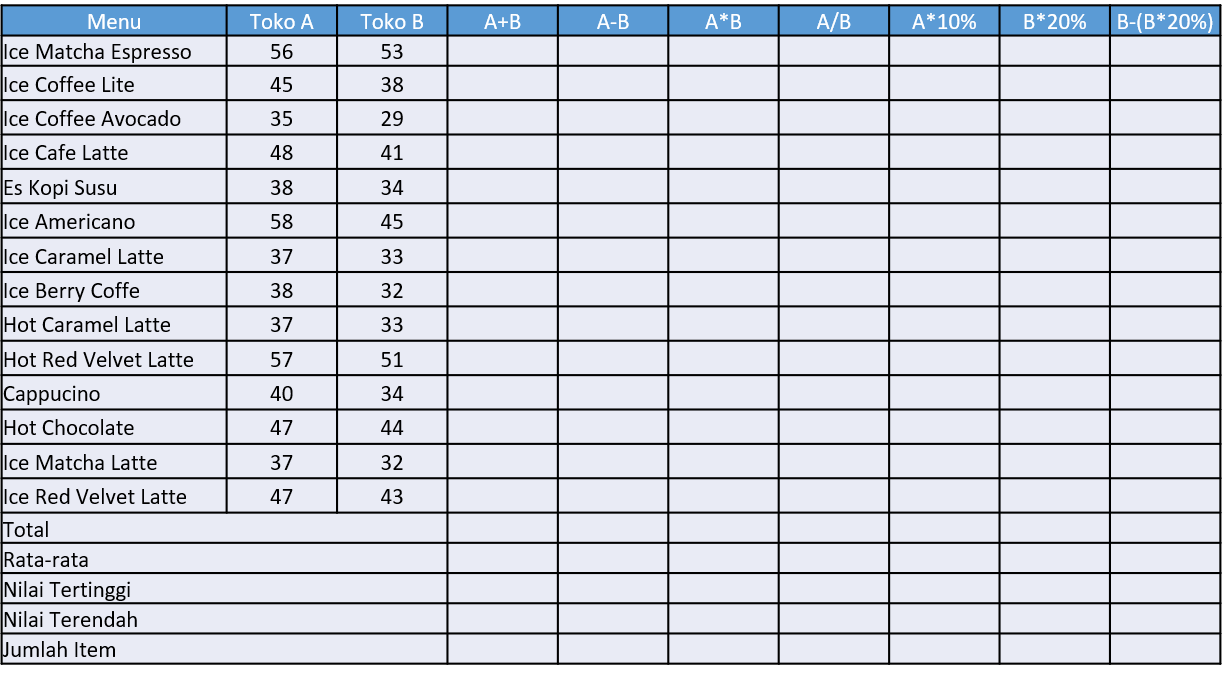
\includegraphics[width=1\linewidth]{images/tabel1} 

}

\caption{Harga Menu Toko A dan B}\label{fig:tabel1}
\end{figure}

\hypertarget{kasus-1.2}{%
\subsection*{Kasus 1.2}\label{kasus-1.2}}
\addcontentsline{toc}{subsection}{Kasus 1.2}

Diberikan daftar Karyawan PT. Kopi Dari Hati \textasciitilde{} Cabang Tangerang, September 2020, pada gambar \ref{fig:tabel2}. Pada bagian ini digunakan fungsi seperti SUM, MIN, AVERAGE, dan MAX.

\begin{figure}

{\centering 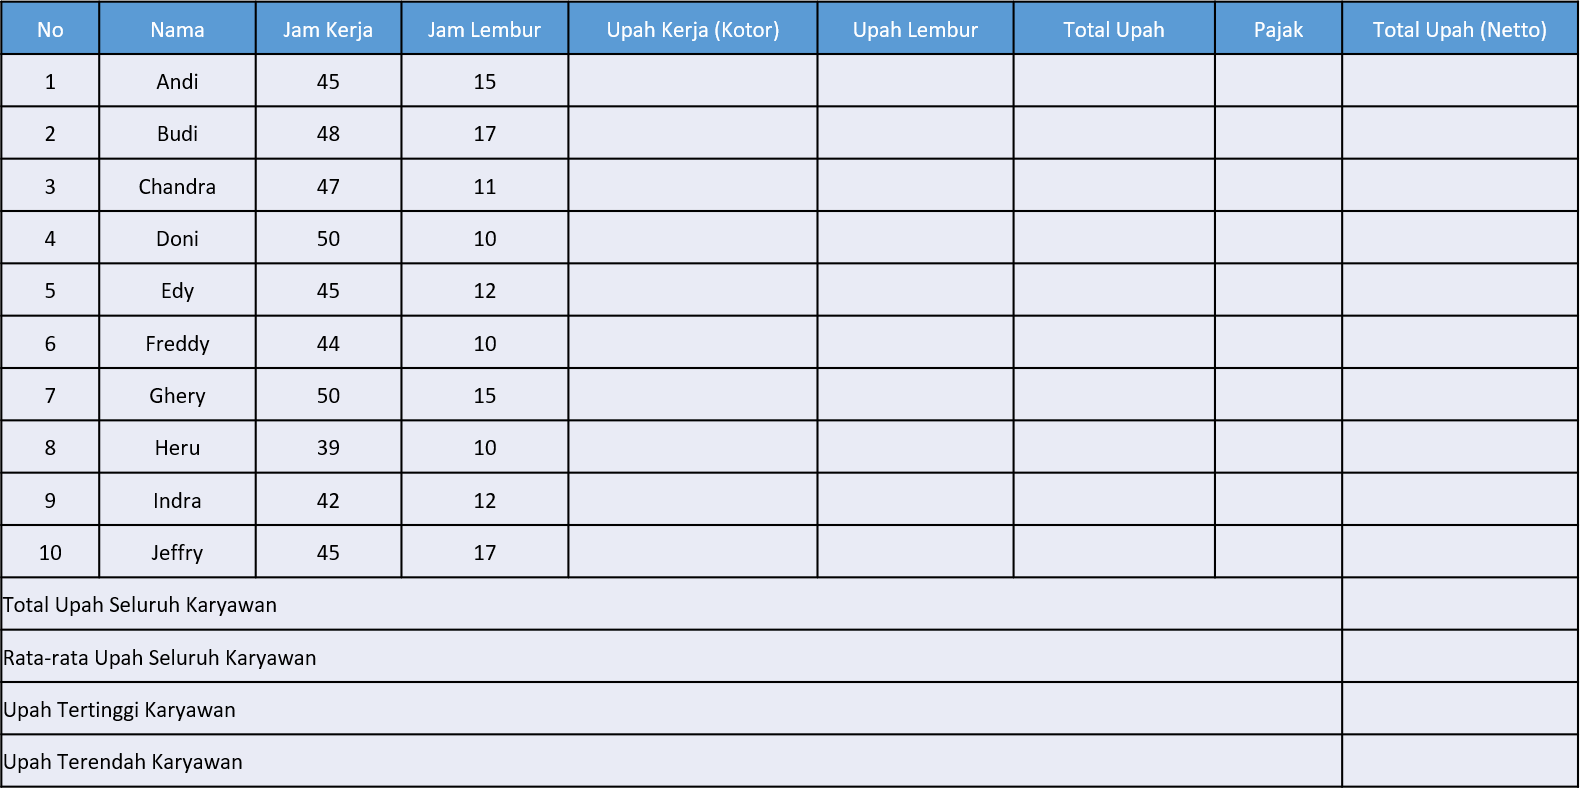
\includegraphics[width=1\linewidth]{images/tabel2} 

}

\caption{Daftar Karyawan}\label{fig:tabel2}
\end{figure}

\textbf{Keterangan:}

\begin{itemize}
\tightlist
\item
  Upah Kerja (Kotor) = Jam Kerja x 25000
\item
  Upah Lembur = Jam Lembur x 30000
\item
  Total Upah = Upah Kerja + Upah Lembur
\item
  Pajak = Total Upah x 5\%
\item
  Total Upah (Netto) = Total Upah -- Pajak
\end{itemize}

\hypertarget{kasus-1.3}{%
\subsection*{Kasus 1.3}\label{kasus-1.3}}
\addcontentsline{toc}{subsection}{Kasus 1.3}

Pada bagian ini anda diharapkan untuk mampu menerapkan Fungsi VLOOKUP untuk mengitung Harga Penjualan Kopi Dari Hati, lihat gambar \ref{fig:tabel3}.

\begin{figure}

{\centering 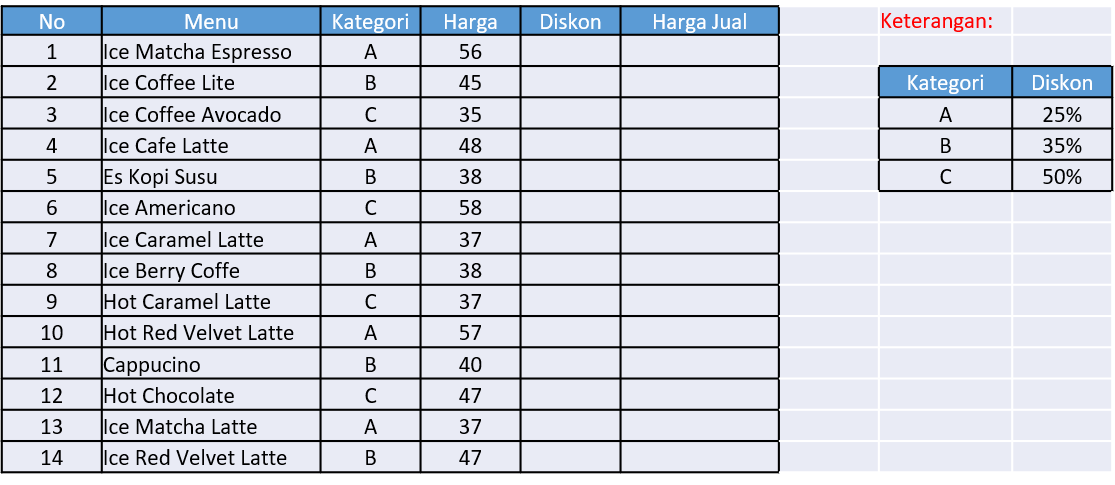
\includegraphics[width=1\linewidth]{images/tabel3} 

}

\caption{Harga Penjualan Kopi Dari Hati}\label{fig:tabel3}
\end{figure}

\textbf{Catatan:}

Vlookup merupakan fasilitas dari Microsoft Excel yakni mengambil data yang ada di tabel lain (tabel Array) berdasarkan data yang sesuai dengan tabel. Selain Vlookup ada juga Hlookup, perbedaannya adalah VLOOKUP digunakan untuk tabel secara Vertikal sedangkan HLOOKUP yaitu pemanggilan tabel array secara Horizontal.

\hypertarget{kasus-1.4}{%
\subsection*{Kasus 1.4}\label{kasus-1.4}}
\addcontentsline{toc}{subsection}{Kasus 1.4}

Pada bagian ini anda diharapkan untuk mampu menerapkan Kombinasi Fungsi VLOOKUP dan HLOOKUP untuk Mengitung Daftar Gaji Karyawan Kopi Dari Hati, lihat gambar \ref{fig:tabel4}.

\begin{figure}

{\centering 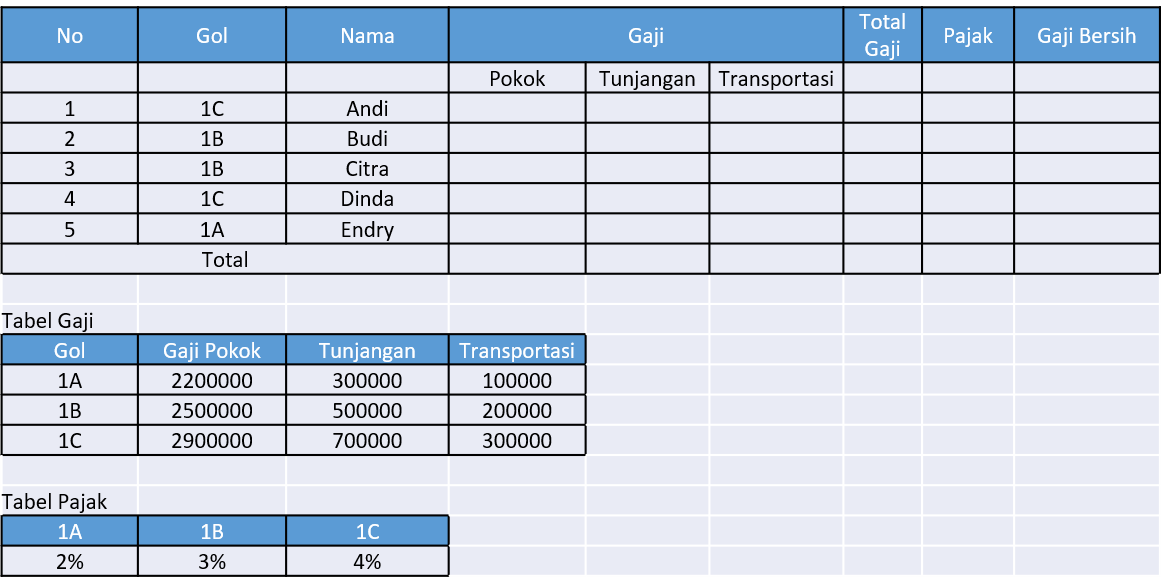
\includegraphics[width=1\linewidth]{images/tabel4} 

}

\caption{Gaji Karyawan Kopi Dari Hati}\label{fig:tabel4}
\end{figure}

\textbf{Keterangan:}

\begin{itemize}
\tightlist
\item
  Untuk gaji sesuai dengan gologan berdasarkan tabel gaji
\item
  Total Gaji =Gaji Pokok+Tunjangan+Transportasi
\item
  Pajak=Total Gaji x Pajak
\item
  Gaji Bersih= Total Gaji -- Pajak
\end{itemize}

\hypertarget{kasus-1.5}{%
\subsection*{Kasus 1.5}\label{kasus-1.5}}
\addcontentsline{toc}{subsection}{Kasus 1.5}

Pada bagian ini anda diharapkan untuk mampu menerapkan Fungsi IF Tunggal dan IF Majemuk untuk melengkapi Daftar Mahasiswa/i Manajemen Universitas Matana 2020 pada gambar \ref{fig:tabel5}.

\begin{figure}

{\centering 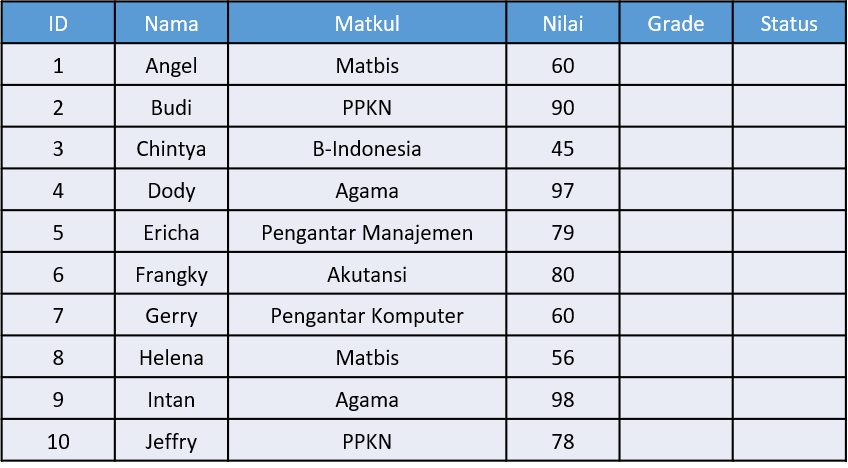
\includegraphics[width=1\linewidth]{images/tabel5} 

}

\caption{Daftar Mahasiswa/i}\label{fig:tabel5}
\end{figure}

\textbf{Keterangan:}

\begin{itemize}
\item
  Grade :

  \begin{itemize}
  \tightlist
  \item
    Grade A for Marks 90 -- 100,
  \item
    Grade B for marks 80 -- 89,
  \item
    Grade C for marks 70 -- 79,
  \item
    Grade D for marks 60 -- 69,
  \item
    Grade E for \textless{} 60
  \end{itemize}
\item
  Status :

  \begin{itemize}
  \tightlist
  \item
    if grade 75 is Complete,
  \item
    if grade \textless{} 75 is Failed
  \end{itemize}
\end{itemize}

\hypertarget{kasus-1.6}{%
\subsection*{Kasus 1.6}\label{kasus-1.6}}
\addcontentsline{toc}{subsection}{Kasus 1.6}

Selesaikan sistem persamaan linear dengan menggunakan Excel.

  \bibliography{book.bib,packages.bib}

\end{document}
